\section{Trådløs kommunikation}
Implementeringen af den trådløse kommunikation 

Der afviges fra det oprindelige design, da opsætningen af Bluetooth kommunikationen i BLE modulet og den nødvendige forståelse for bluetooth bibliotekerne er meget omfattende. 


Dertil implementeres en mere simpel løsning, hvor der benyttes to PSoC 4 M-Series Prototyping Kit board, der ses af \autoref{fig:PSoC_4200}. Denne mikrokontroller består at to elementer, hvor KigProg er programmer og debugger, og PSoC 4200M der koden eksekveres. 
Boards er alene ikke i stand til trådløs kommunikation, og er derfor begge blevet udstyret med EZ-BLE PRoC modul der muliggør BLE kommunikation.

\begin{figure}[H]
	\centering
	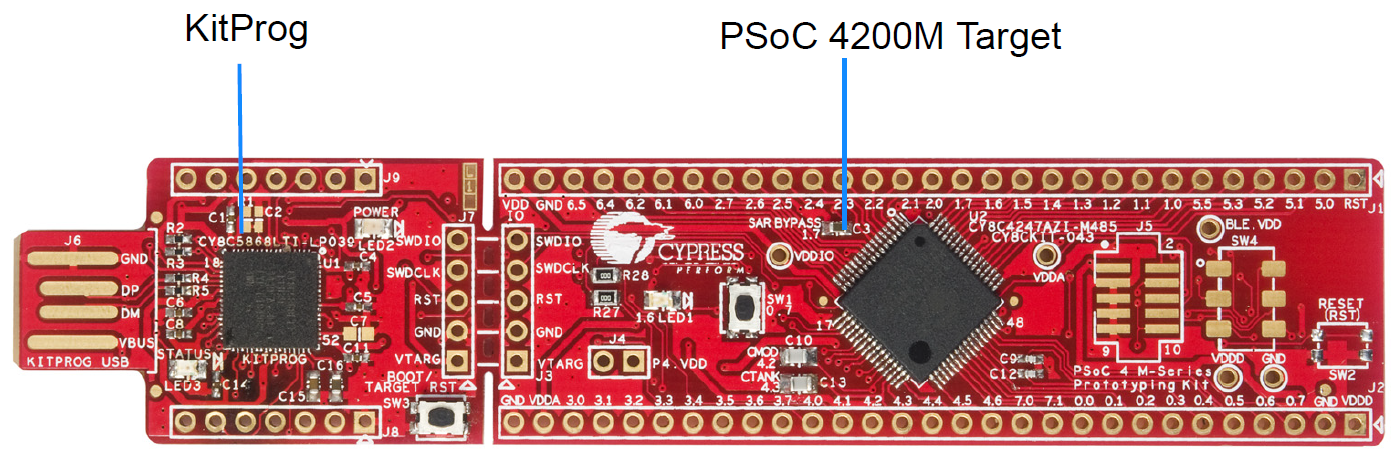
\includegraphics[width=1\textwidth]{figure/PSoC_4200_opdelt.png}
	\caption{CY8CKIT-043 PSoC 4 M-Series Prototyping Kit\citep{cypress42015}.}
	\label{fig:PSoC_4200}
\end{figure}

Begge 





\begin{figure}[H]
	\centering
	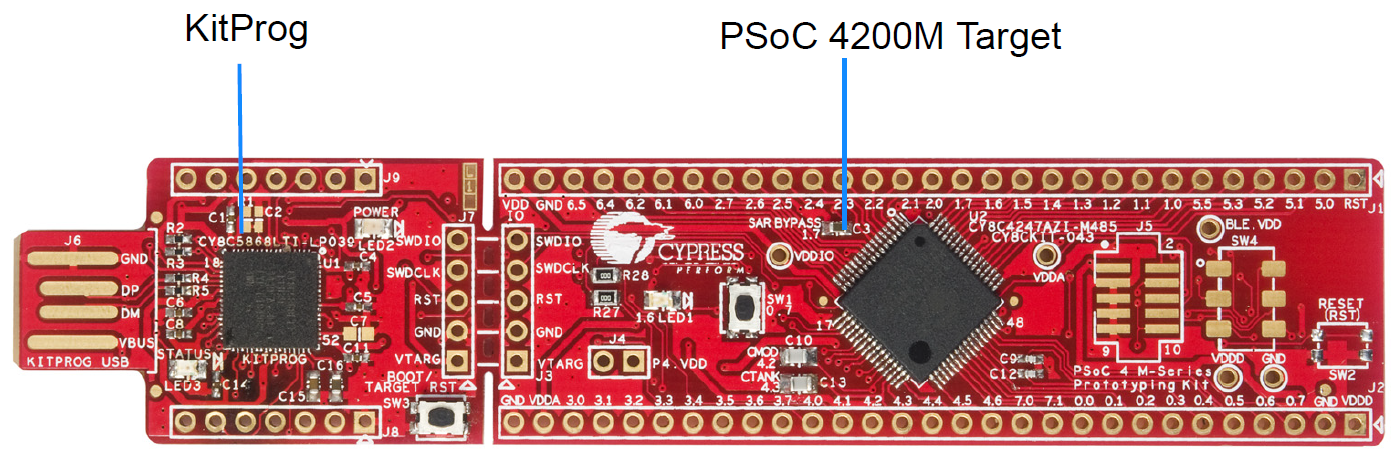
\includegraphics[width=1\textwidth]{figure/PSoC_4200_opdelt.png}
	\caption{CIllustration af kommunikation mellem mikrokontroller og computer.}
	\label{fig:PSoC_4200}
\end{figure}